%% Ankur Sinha

%% packages %%
% support for coloured text
\usepackage{xcolor}
% moreland colour palette:
% https://github.com/Gnuplotting/gnuplot-palettes/blob/master/moreland.pal
% create: blue
\definecolor{moreland1}{HTML}{3b4cc0}
%visualise
\definecolor{moreland2}{HTML}{688aef}
%validate
\definecolor{moreland3}{HTML}{99baff}
%simulate
\definecolor{moreland4}{HTML}{c9d8ef}
%fit
\definecolor{moreland5}{HTML}{edd1c2}
%share
\definecolor{moreland6}{HTML}{f7a789}
%reuse
\definecolor{moreland7}{HTML}{e36a53}
% extra: red
\definecolor{moreland8}{HTML}{b40426}

% set 1 colour palette
% https://github.com/Gnuplotting/gnuplot-palettes/blob/master/set1.pal
% red
\definecolor{set11}{HTML}{E41A1C}
% blue
\definecolor{set12}{HTML}{377EB8}
% green
\definecolor{set13}{HTML}{4DAF4A}
% purple
\definecolor{set14}{HTML}{984EA3}
% orange
\definecolor{set15}{HTML}{FF7F00}
% yellow
\definecolor{set16}{HTML}{FFFF33}
% brown
\definecolor{set17}{HTML}{A65628}
% pink
\definecolor{set18}{HTML}{F781BF}

% IPA
\usepackage{tipa}
\usepackage[scale=2]{ccicons}
\usepackage{amssymb}
\usepackage{tikz}
\usetikzlibrary{arrows.meta, arrows, positioning}
\usepackage{jneurosci}
\usepackage{subcaption}
\usepackage[T1]{fontenc}
\usepackage[utf8]{inputenc}
\usepackage[style=nature,backend=biber,autocite=footnote]{biblatex}
\addbibresource{/home/asinha/Documents/01_Readables/00_research_papers/bibliography/masterbib.bib}
\usepackage{roboto}
% for strike through
\usepackage[normalem]{ulem}
% links, urls, refs
\usepackage{hyperref}
\hypersetup{colorlinks,linkcolor=Green,urlcolor=set18}
% graphics
\usepackage{graphicx}
% algorithm
\usepackage{algorithmic}
\usepackage{textcomp}
\usepackage{wrapfig}
\usepackage{textgreek}
\usepackage{euler}
\usepackage{tabularx}
\usepackage{booktabs}
\usepackage{minted}
\usepackage{csquotes}
% beamer theme
% use defaults for theme
\usetheme{moloch}
% for footnotes
% https://tex.stackexchange.com/questions/683533/beamer-theme-metropolis-does-not-allow-different-font-size-for-fullcite/683540#683540
\setbeamerfont{bibliography entry title}{size=}
\setbeamerfont{bibliography entry author}{size=}
\setbeamerfont{bibliography entry location}{size=}
\setbeamerfont{bibliography entry note}{size=}
%\usetheme[numbering=fraction,sectionpage=progressbar,subsectionpage=progressbar,progressbar=frametitle]{metropolis}
%\usefonttheme[onlymath]{serif}
\setbeamerfont{footnote}{size=\tiny}
\setbeamerfont{caption}{size=\tiny}
\setbeamercolor{alerted text}{fg=Green}
\setbeamerfont{note page}{size=\small}
\setbeamercolor{alerted text}{fg=set15}
\setbeamercolor{progress bar}{fg=set18}
\setbeamercolor{title separator}{fg=set18}
\setbeamercolor{frametitle}{bg=moreland1}

\renewcommand{\figurename}{}

% Not needed in metropolis, but in general footnote citation fixes: https://tex.stackexchange.com/questions/44217/how-can-i-stop-footcite-from-hijacking-my-beamer-columns
% how to use multiple references to the same footnote: https://tex.stackexchange.com/questions/27763/beamer-multiple-references-to-the-same-footnote

% Disable footnoterule
\renewcommand{\footnoterule}{}
\renewcommand*{\bibfont}{\tiny}

%% title %%
\title{The NeuroML ecosystem for standardised multi-scale modelling in neuroscience}
\author[Ankur Sinha]{Ankur Sinha\\Silver Lab\\Department of Neuroscience, Physiology, \& Pharmacology\\University College London}
\date{2024-02-26}

%% document begins %%
\begin{document}


% title frame %%
\begin{frame}
  \titlepage{}
\end{frame}
%% Three slides for 5 minutes seems good
%% So, 30 slides at most for 50 minutes

% Why is biophysically detailed modelling important?
% Why are standards necessary?
%\section{Biophysically detailed models and standards}
\begin{frame}[c]
  \frametitle{An understanding of the brain}
  \begin{columns}
    \begin{column}{0.5\textwidth}
      \begin{figure}[h]
        \centering
        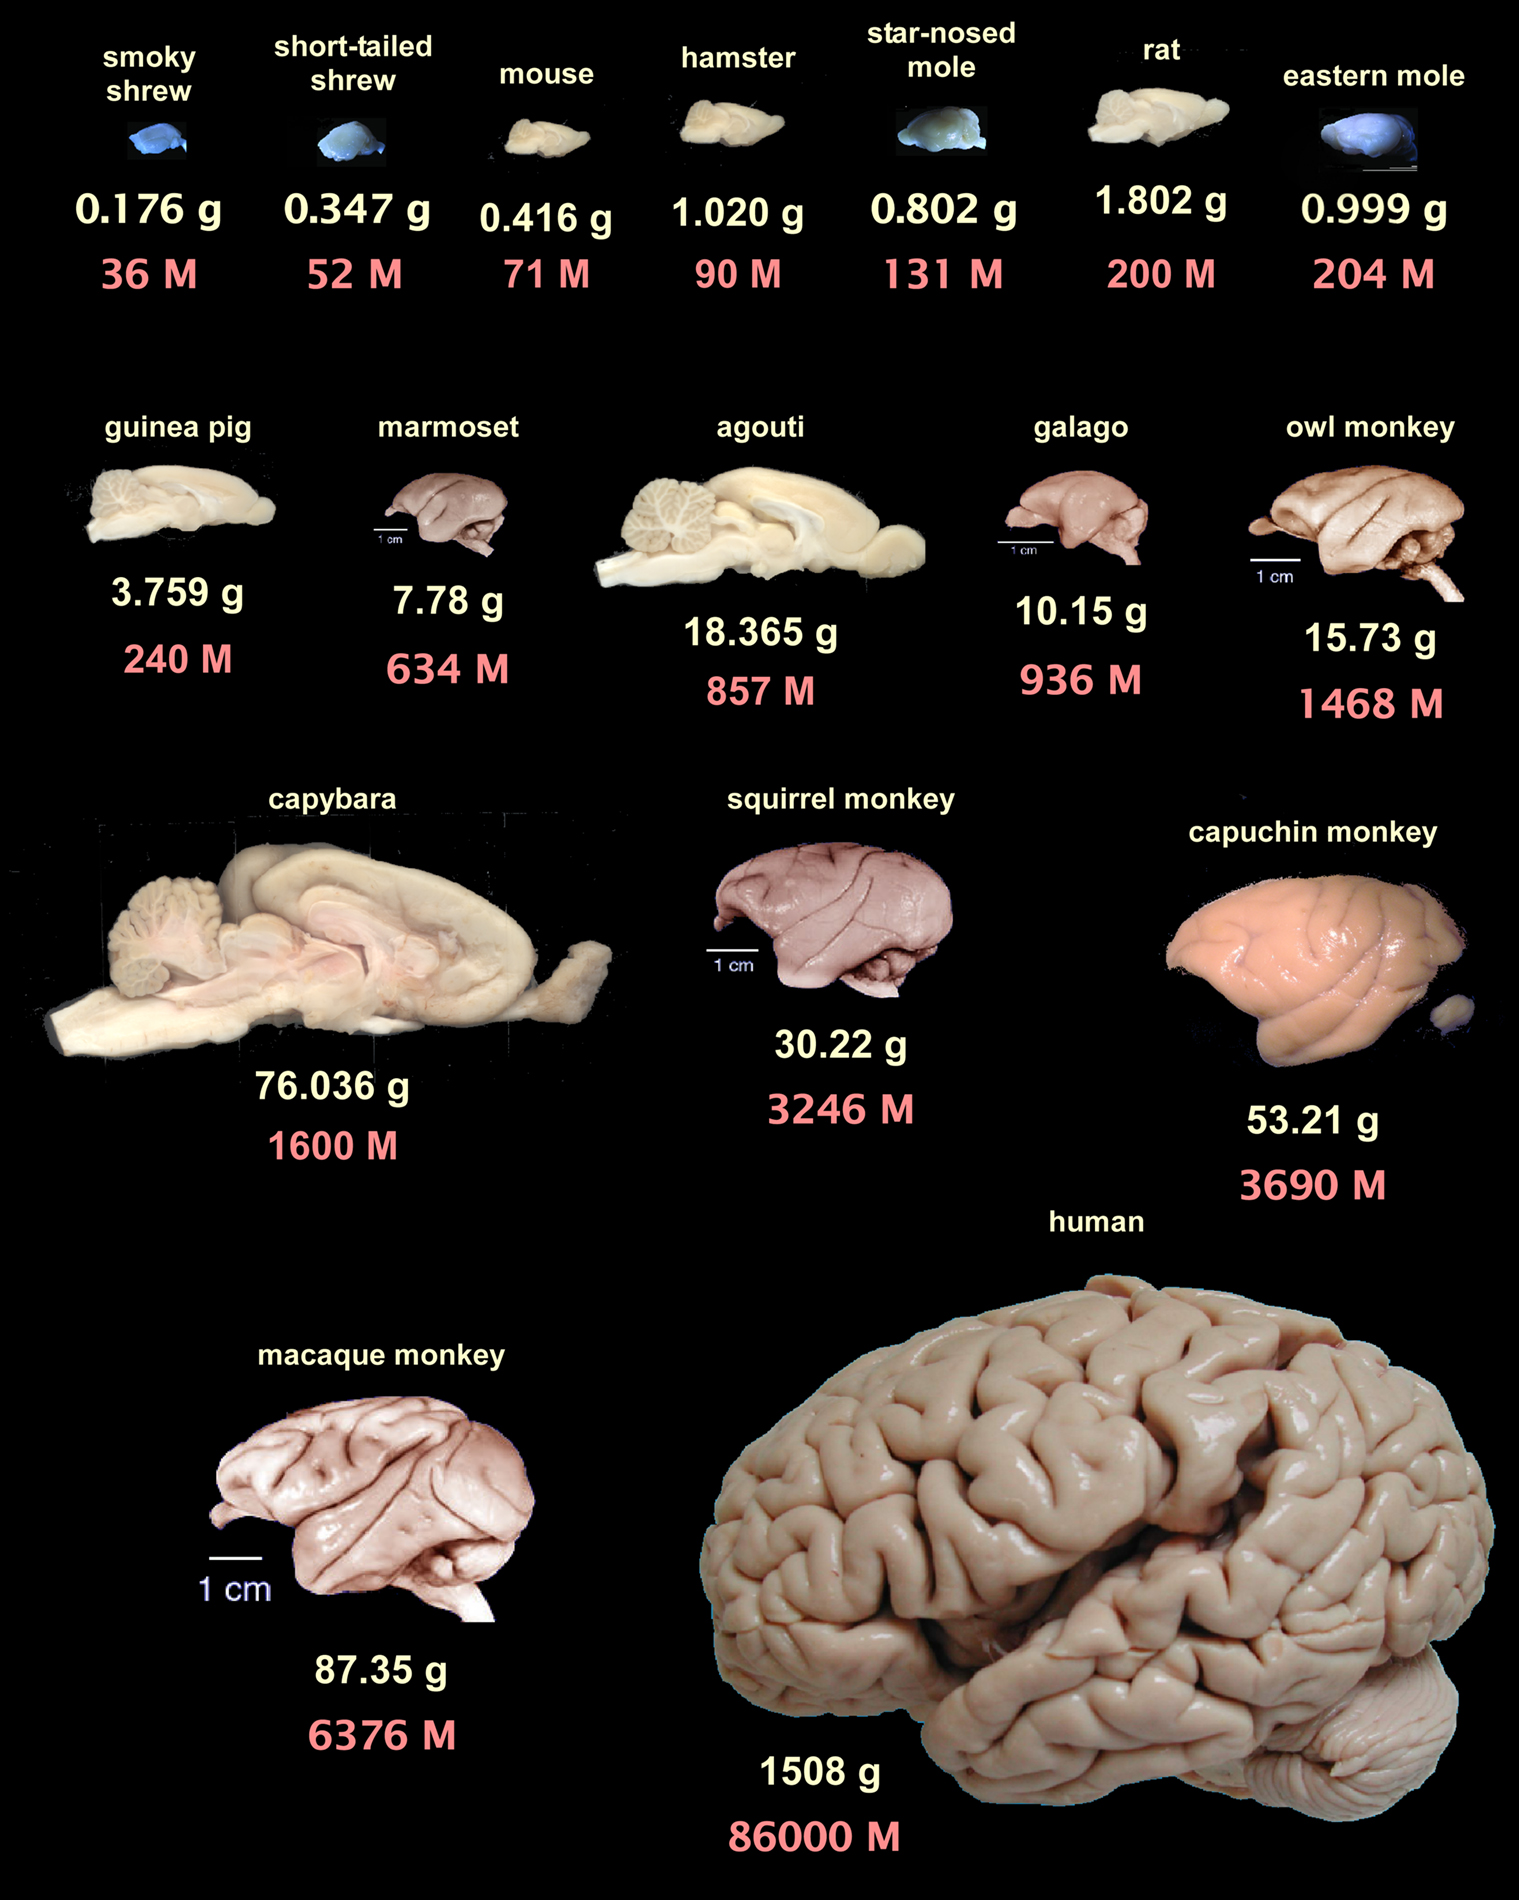
\includegraphics[width=\textwidth]{99_images/brain-sizes.jpg}
      \end{figure}
    \end{column}
    \begin{column}{0.5\textwidth}
      \begin{itemize}
        \only<1>{%
          \item<1> \alert{86B} neurons
          \item<1> also similar number of \alert{glia}
        }
        \only<2>{%
          \item<2> sensing
          \item<2> cognition
          \item<2> action
        }
      \end{itemize}
    \end{column}
  \end{columns}
  \vspace{0.2cm}
  \footnotetext[1]{{\tiny{\fullcite{HerculanoHouzel2009}}}}
\end{frame}
\note[enumerate]{%
  \item The most recent estimate puts the number of neurons in the human brain at 86B.
  \item Experiments provide us with direct information.
  \item They study the brain at different levels.
  \item There's no right level. It depends on the question being investigated.
}
\begin{frame}[c]{The brain: diversity of neurons}
  \begin{figure}[h]
    \centering
    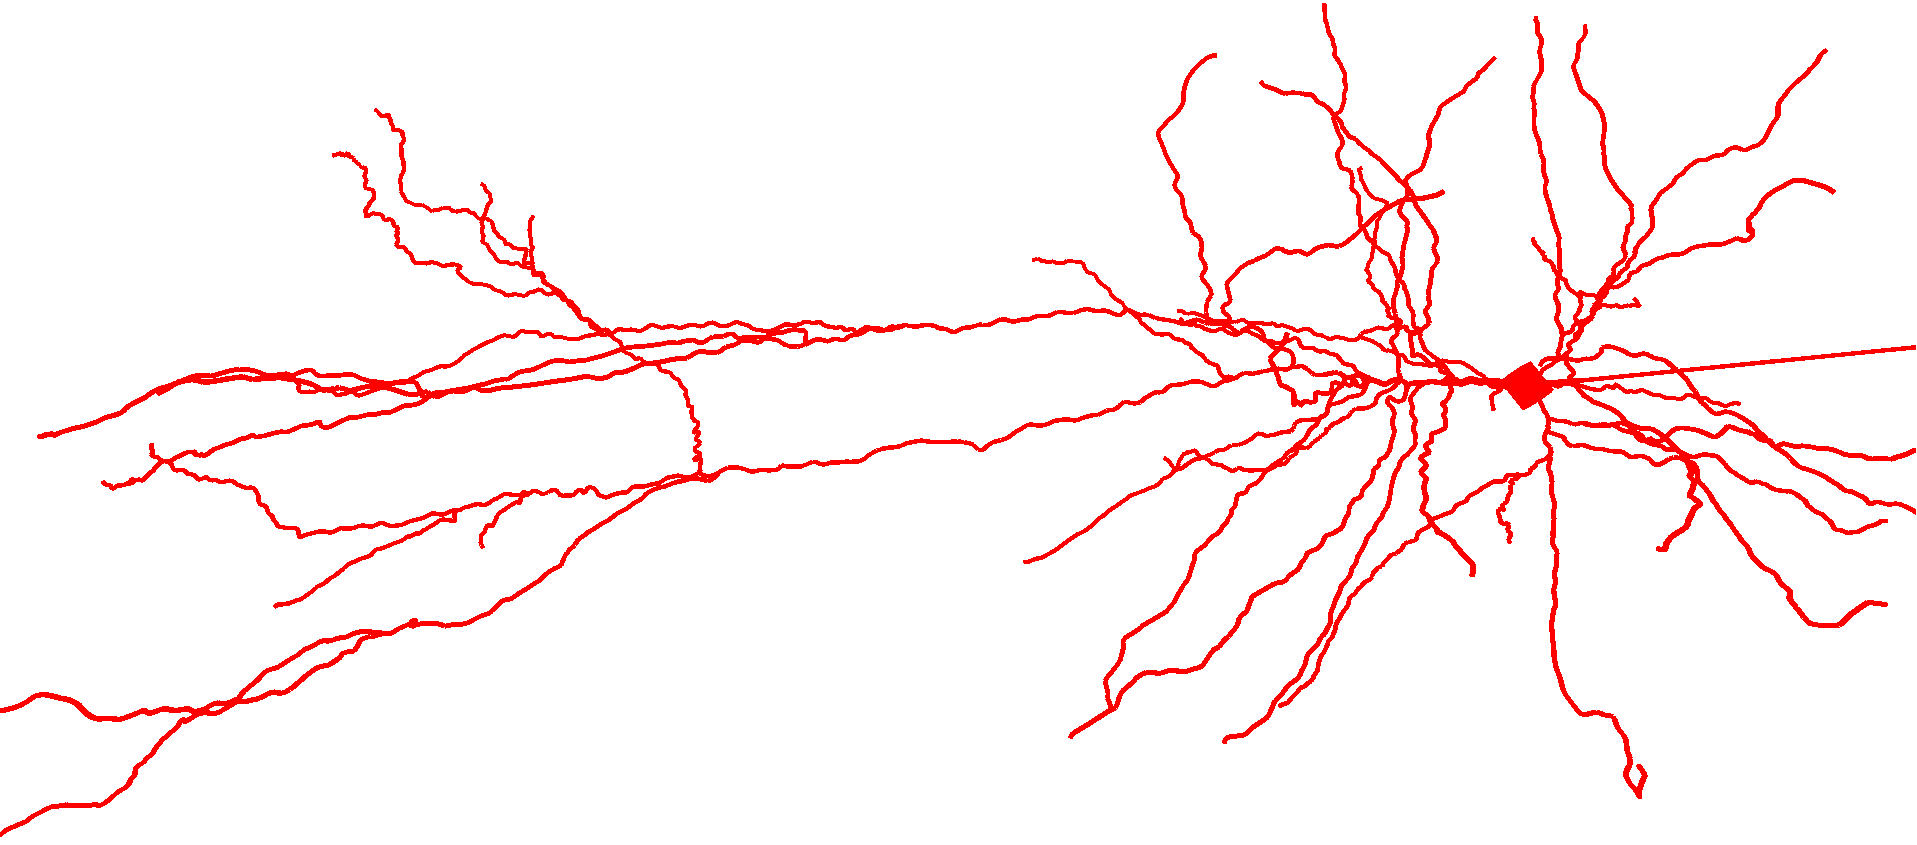
\includegraphics[width=0.5\linewidth,angle=-90]{99_images/HL23PYR-red}
    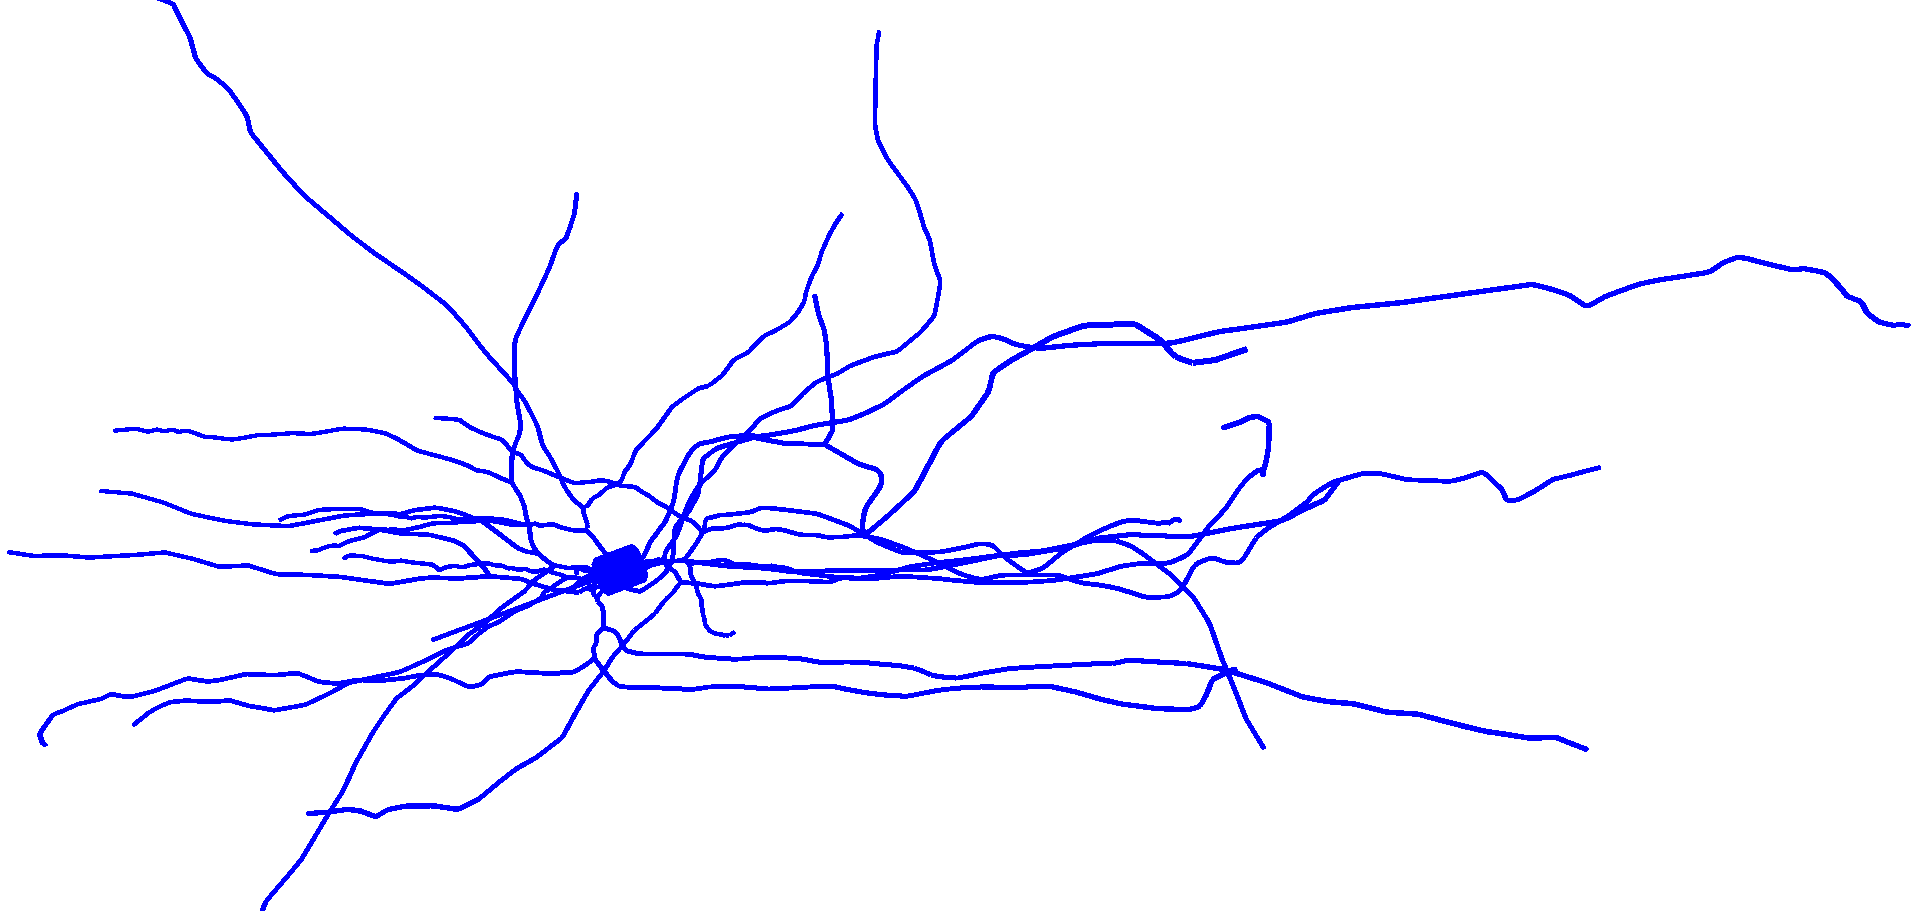
\includegraphics[width=0.5\linewidth,angle=-90]{99_images/HL23PV}
  \end{figure}
  \note[item]{Neurons in the brain are diverse. Here we show different morphologies, but they also differer by other parameters---protein composition and so on.}
  \footnotetext[1]{\fullcite{Yao2022}}
\end{frame}
\begin{frame}[c]
  \frametitle{Experiments provide a window into the brain}
  Multiple scales of experiments goes here
\end{frame}
\note[enumerate]{%
\item There is so much data out there now, as we embrace Open Science.
\item Models/theory are necessary for:
\item combining independent experimental results into unified theories
\item exploring these complex systems across wider range of conditions
\item generating new testable hypotheses
\item RNNs are appropriate for lots of projects, for example.
\item So are whole brain neural mass models.
\item But, to really understand the underlying mechanisms that give rise to emergent behaviour, we must model the brain at biophysically detailed levels.
}
\begin{frame}[c]
  \frametitle{A \emph{mechanistic} understanding of the brain}
  Figure showing multiple scales of modelling goes here.
\end{frame}
\note[enumerate]{%
\item There is so much data out there now, as we embrace Open Science.
\item Models/theory are necessary for:
\item combining independent experimental results into unified theories
\item exploring these complex systems across wider range of conditions
\item generating new testable hypotheses
\item RNNs are appropriate for lots of projects, for example.
\item So are whole brain neural mass models.
\item But, to really understand the underlying mechanisms that give rise to emergent behaviour, we must model the brain at biophysically detailed levels.
}
\begin{frame}[c]
  \frametitle{The model life cycle}
  \begin{itemize}
    \item tweaked version of life cycle figure from paper goes here.
    \item remove NeuroML, add data
  \end{itemize}
\end{frame}
\note[enumerate]{%
\item The figure shows a simplified model life cycle. Can be much more complex in practice.
\item Lots of tools out there for each step.
\item But there's are issues---fragmentation, lack of interoperability, so many APIs.
}
\begin{frame}[c]
  \frametitle{Standards enable FAIR neuroscience}
  \begin{itemize}
    \item NWB/BIDS for data
    \item NeuroML/SBML etc.\ for modelling
    \item Add logos
  \end{itemize}
\end{frame}
\note[enumerate]{%
\item Standards allow the representation of data and models in specific, agreed formats.
\item They're not neuroscience specific, of course---even programming languages have standards.
\item More importantly, if one knows what the data is going to look like, one can then develop tools and APIs around it.
\item And instead of everyone writing a tool for their own standard, every tool anyone writes for the one standard can be used with everyone's data.
}
\begin{frame}[c]
  \frametitle{But, too many standards?}
  \begin{itemize}
    \item XKCD here.
  \end{itemize}
\end{frame}
\note[enumerate]{%
\item In neuroscience, we're fortunate enough to not have the issue of having too many standards.
\item There are only a few standards in biophysically detailed modelling, and as we'll see, we ensure that these few remain interoperable.
}
%\section{NeuroML}
\begin{frame}[c]
  \frametitle{NeuroML}
  \begin{itemize}
    \item Introduction to NeuroML.
  \end{itemize}
\end{frame}
\begin{frame}[c]
  \frametitle{NeuroML: scope}
  \begin{itemize}
    \item Figure 2 from paper
  \end{itemize}
\end{frame}
\begin{frame}[c]
  \frametitle{NeuroML: software ecosystem}
  \begin{itemize}
    \item Figure 3
  \end{itemize}
\end{frame}
\begin{frame}[c]
  \frametitle{NeuroML: software ecosystem: core tools}
  \begin{itemize}
    \item Figure 4
  \end{itemize}
\end{frame}
\begin{frame}[c]
  \frametitle{NeuroML: create models}
  \begin{itemize}
    \item Figure 5
    \item Code example
  \end{itemize}
\end{frame}
\begin{frame}[c]
  \frametitle{NeuroML: validate models}
  \begin{itemize}
    \item Figure 6
  \end{itemize}
\end{frame}
\begin{frame}[c]
  \frametitle{NeuroML: visualise models}
  \begin{itemize}
    \item Figure 7
    \item Figure 8
    \item Figure 9
  \end{itemize}
\end{frame}
\begin{frame}[c]
  \frametitle{NeuroML: simulate models}
  \begin{itemize}
    \item Example simulation: neuron/netpyne
  \end{itemize}
\end{frame}
\begin{frame}[c]
  \frametitle{NeuroML: fit models}
  \begin{itemize}
    \item Figure from docs
    \item Mention inspyred
  \end{itemize}
\end{frame}
\begin{frame}[c]
  \frametitle{NeuroML: share and re-use models}
  \begin{itemize}
    \item GitHub, OSBv1, OSBv2, NeuroML-DB
  \end{itemize}
\end{frame}
%\section{Under the hood}
\begin{frame}[c]
  \frametitle{NeuroML: the standard}
  \begin{itemize}
    \item Schema, component types
  \end{itemize}
\end{frame}
\begin{frame}[c]
  \frametitle{NeuroML: the APIs}
  \begin{itemize}
    \item Python API
  \end{itemize}
\end{frame}
\begin{frame}[c]
  \frametitle{NeuroML: LEMS}
  \begin{itemize}
    \item LEMS, advantages
  \end{itemize}
\end{frame}
\begin{frame}[c]
  \frametitle{NeuroML: Documentation}
  \begin{itemize}
    \item Jupyterbook
  \end{itemize}
\end{frame}
\begin{frame}[c]
  \frametitle{NeuroML: projects}
  \begin{itemize}
    \item GSoC, Outreachy, good computer science students
  \end{itemize}
\end{frame}
\end{document}
